%%%%% Single page layout:
%%%%% ----------------------------------------------------
%\documentclass[12pt, a4paper,draft]{report}
\documentclass[12pt, a4paper]{report}
\setlength\textwidth{160mm}
\setlength\textheight{247mm}
\setlength\oddsidemargin{0mm}
\setlength\evensidemargin{0mm}
\setlength\topmargin{0mm}
\setlength\headsep{0mm}
\setlength\headheight{0mm}
\let\openright=\clearpage
% Overfull statements
\pretolerance=150
\setlength{\emergencystretch}{3em}
% Overfull end

\usepackage[utf8]{inputenc}


%%% Additional useful packages
%%% ----------------------------------------------------------------
\usepackage{array}
\usepackage{amsmath}  
\usepackage{amssymb}
\usepackage{amsfonts}
\DeclareFontFamily{OT1}{pzc}{}
\DeclareFontShape{OT1}{pzc}{m}{it}{<-> s * [0.900] pzcmi7t}{}
\DeclareMathAlphabet{\mathpzc}{OT1}{pzc}{m}{it}
\usepackage{amsthm}      
\usepackage[ruled,algochapter]{algorithm2e}
\usepackage{algorithmic}
\usepackage{bm}
\usepackage[mathscr]{euscript}
\usepackage{graphicx}       
\usepackage{psfrag}         
\usepackage{fancyvrb}    
\usepackage{float}
\usepackage{ltablex}
\usepackage[square,sort,comma,numbers]{natbib}        
\usepackage{bbding}         
\usepackage{dcolumn}        
\usepackage{booktabs} 
\usepackage{multirow}
\usepackage{paralist}       
\usepackage{indentfirst}    
\usepackage[nottoc,notlof,notlot]{tocbibind}
\usepackage{url}
\usepackage{tabularx}
\usepackage{subcaption}
\usepackage[unicode]{hyperref}
\usepackage{xcolor}

\hypersetup{pdftitle=LiDAR obstacle detection and avoidance, 
            pdfauthor=Alojz Gomola,
            colorlinks=false,
            urlcolor=blue,
            pdfstartview=FitH,
            pdfpagemode=UseOutlines,
            pdfnewwindow,
            breaklinks
          }
\usepackage{array}
\newcolumntype{L}[1]{>{\raggedright\let\newline\\\arraybackslash\hspace{0pt}}m{#1}}
\newcolumntype{C}[1]{>{\centering\let\newline\\\arraybackslash\hspace{0pt}}m{#1}}
\newcolumntype{R}[1]{>{\raggedleft\let\newline\\\arraybackslash\hspace{0pt}}m{#1}}         
\newcolumntype{B}{X}
\newcolumntype{S}[1]{>{\hsize=#1\textwidth}X}

\newcommand{\FIGDIR}{./Pics}    %%% directory containing figures
\newcommand{\twolinecellr}[2][r]{%
  \begin{tabular}[#1]{@{}r@{}}#2\end{tabular}}
\theoremstyle{plain}
\newtheorem{theorem}{Theorem}
\newtheorem{lemma}[theorem]{Lemma}
\newtheorem{proposition}[theorem]{Proposition}

\theoremstyle{plain}
\newtheorem{definition}{Definition}
\newtheorem{problem}{Problem}
\newtheorem{example}{Example}
\newtheorem{assumption}{Assumption}

\theoremstyle{remark}
\newtheorem*{corollary}{Corollary}
\newtheorem*{note}{Note}




\newenvironment{dokaz}{
  \par\medskip\noindent
  \textit{Proof}.
}{
\newline
\rightline{\SquareCastShadowBottomRight}
}

\newenvironment{constraints}[1]{
  \par\medskip\noindent
  \textit{Constraints #1} \\
}{
\newline
\rightline{\SquareCastShadowBottomRight}
}


%\bibliographystyle{plainnat}     %% Author (year) style
\bibliographystyle{unsrt}        %% [number] style
\setcitestyle{square}

% Section  3.7 Challenge list
\newif\ifproblemchallenge   %# Build block for problem challenges
\problemchallengetrue       %# Show comments


\title{Dissertation thesis}
\author{Alojz Gomola}
\date{February 2019}

%%%%% ------------------------------------------------------------
\DefineVerbatimEnvironment{PCinout}{Verbatim}{fontsize=\small, frame=single}



\newcommand{\R}{\mathbb{R}}
\newcommand{\N}{\mathbb{N}}

\DeclareMathOperator{\pr}{\textsf{P}}
\DeclareMathOperator{\E}{\textsf{E}\,}
\DeclareMathOperator{\var}{\textrm{var}}
\DeclareMathOperator{\sd}{\textrm{sd}}


\newcommand{\T}[1]{#1^\top}        

\newcommand{\goto}{\rightarrow}
\newcommand{\gotop}{\stackrel{P}{\longrightarrow}}
\newcommand{\maon}[1]{o(n^{#1})}
\newcommand{\abs}[1]{\left|{#1}\right|}
\newcommand{\dint}{\int_0^\tau\!\!\int_0^\tau}
\newcommand{\isqr}[1]{\frac{1}{\sqrt{#1}}}
\newcommand{\norm}[1]{\left\lVert#1\right\rVert}


\newcommand{\pulrad}[1]{\raisebox{1.5ex}[0pt]{#1}}
\newcommand{\mc}[1]{\multicolumn{1}{c}{#1}}
\newcommand{\TBD}[1]{\color{red}\emph{--TBD:}#1\color{black}}

\begin{document}
\setcounter{chapter}{6}
\setcounter{section}{3}
    %06-04 Static Obstacles and Constraints
    \cleardoublepage
\section{\secState{R}Static Obstacles and Constraints}\label{s:staticObstacles}
    
\paragraph{Introduction:} The \emph{static obstacles} were used in original concept \cite{gomola2017probabilistic}, the \emph{Avoidance Grid} and \emph{Movement Automaton} were repurposed to enable \emph{finite time deterministic} avoidance. An \emph{Constraint based path search} and \emph{obstacle modeling} is summarized in \cite{hentenryck2009constraint}.

This section is handling basic problems of \emph{static obstacle} detection and its focused on following real-world fixed position threats:
\begin{enumerate}
    \item \emph{Static Obstacles} - detected by LiDAR sensor or fused from \emph{Obstacle Map} information source.
    
    \item \emph{Geo-fencing Areas} - defined by offline/online information source as permanent flight restriction zones. There is usually no physical obstacle. The space is considered as \emph{hard/soft constraint}.
    
    \item \emph{Long-term bad weather Areas} - the \emph{weather} is changing often (hour period), there are \emph{weather events}  which lasts for \emph{hours} or \emph{days}.
\end{enumerate}


\paragraph{Changing Scanning Density of LiDAR:} A LiDAR sensor is scanning in conic section given by $distance Range$, $horizontal Range$, $vertical Range$, where distance range is in interval $[0,maxDistance]$, horizontal offset range is in $[-pi,pi]$, and vertical offset range is in $[\varphi_s, \varphi_e]$.  

Let say that $\text{d} horizontal^\circ, \text{d} vertical^\circ$ is unitary angle offset in which one LiDAR send and return is executed. That means the \emph{LiDAR} ray is sent every $\text{d} horizontal^\circ, \text{d} vertical^\circ$ offset movement. The \emph{LiDAR} ray density is decreasing with \emph{distance offset}. The same amount of \emph{LiDAR} rays passes trough $cell_{i,j,k}$ in Avoidance Grid.

The surface of area given by some distance d, and unitary offsets$\partial horizontal^\circ, \text{d} vertical^\circ$  is changing with $distance$. The minimal triggering area of object surface is not changing. This fact has an impact on count of the hits on object surface. 

The example is given in (fig. \ref{fig:P01CountOfLiDARHits}) where we have two identical objects (red circle) in distances 5 and 10 meters. The closer object consumes 5 LiDAR beam hits and the farther object consumes only 3 LiDAR beam hits. The probability of obstacle encounter is remaining the same for closer and farther object. The \emph{detected obstacle rate} assessment should return the same  detected obstacle collision rate for objects with same scanned surface (with different LiDAR ray hit count).

\begin{figure}[H]
    \centering
    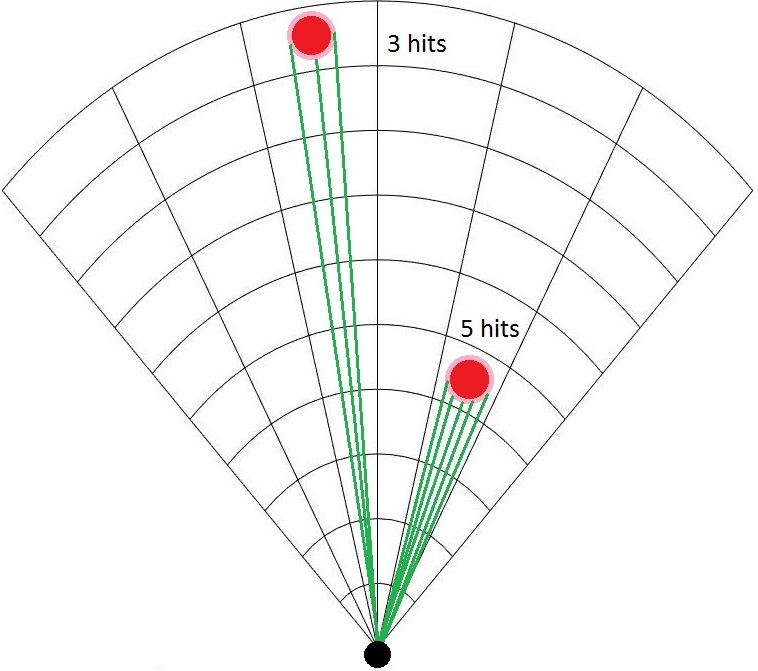
\includegraphics[width=0.7\textwidth]{\FIGDIR/TE051CountOfLiDARHits}
    \caption{Different count of LiDAR hits with different distance from UAS.}
    \label{fig:P01CountOfLiDARHits}
\end{figure}


\paragraph{Map and Detected Obstacles Fusion:} The concept of \emph{offline/online obstacle map} is mandatory in modern obstacle avoidance systems and increases the safety of navigation/avoidance path. The \emph{older} concept was considering only LiDAR reading or \emph{real-time sensor readings} in general \cite{gomola2017probabilistic}. 

\begin{figure}[htbp]
    \centering
    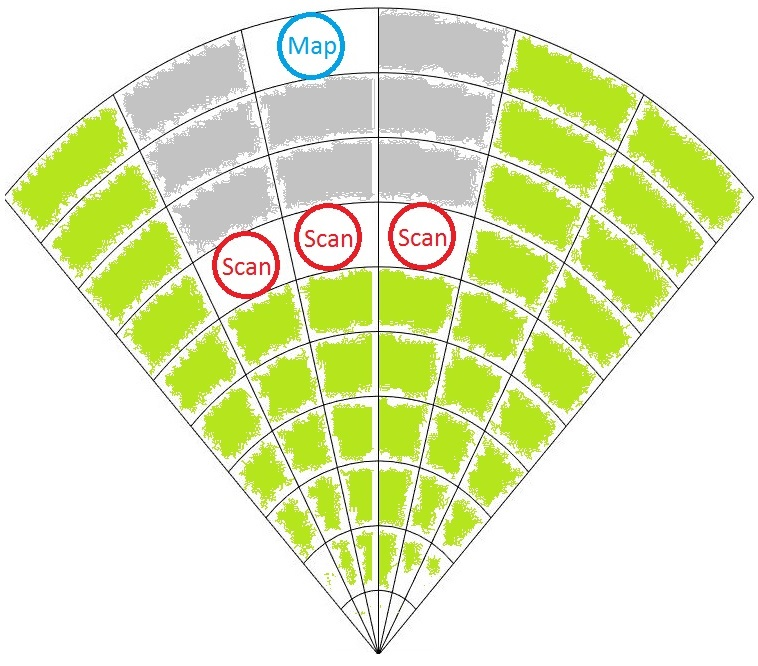
\includegraphics[width=0.7\textwidth]{\FIGDIR/TE053OvershadowedMapobstacle}
    \caption{Overshadowed map obstacle by detected obstacles.}
    \label{fig:P02OvershadowedMapobstacle}
\end{figure}

\newpage\noindent The fusion of real time sensor readings and obstacle map (prior knowledge) is required. Data fusion of these two sources is strongly depending on visibility property, because there are three basic scenarios:

\begin{enumerate}
    \item \emph{Dual detection} - the obstacle is marked on the map and detected by sensory system at some point of the time (older concept works).
    
    \item \emph{Hindered vision} - the detected obstacles are hindering vision to map obstacle therefore map obstacle uncertainty arises (older concept fails). 
    
    \item \emph{False-positive map} - map obstacle occupied space is visible by sensory system, but negative detection is returned. Therefore the map is giving \emph{false-positive} information.
\end{enumerate}

\noindent The second case is given in fig. \ref{fig:P02OvershadowedMapobstacle}, where map obstacle (blue circle) is overshadowed by three scanned obstacles (red circle). The visible space is denoted by green fill, the invisible space is denoted by gray fill. 
    	\subsection{(R) Detected obstacles}\label{s:detectedObstacles}
\paragraph{Idea:} The \emph{visibility} inside avoidance grid and \emph{obstacle} probability are interconnected for most ranging sensors (ex. LiDAR). The goal of this section is to introduce \emph{visibility hindrance} concept which includes space uncertainty assessment and detected obstacle  processing.

\paragraph{Detected Obstacle Rating:} The \emph{detected obstacle rating} defines UAS chances to encounter detected obstacle in avoidance grid $cell_{i,j,k}$. Final \emph{detected obstacle rating} is merged information (eq. \ref{eq:detectedObstacleRatingForCell}). The \emph{sensor field} can contain \emph{multiple} \emph{static obstacle sensors}.

\paragraph{Detected Obstacle Rate for LiDAR:},Lets have only one sensor set as homogeneous two axis rotary LiDAR. For one $cell_{i,j,k}$ there exists set of passing LiDAR beams:

\begin{equation}\label{eq:lidarRaysTroughCell}
    lidar Rays(cell_{i,j,k})=
    \left\{
        \begin{aligned}
        \left[
            \begin{gathered}
                horizontal^\circ\in horizontal Offsets,\\
                vertical^\circ\in vertical Offsets
            \end{gathered}
        \right]\in\R^2:&\\
        horizontal^\circ\in cell_{i,j,k}.horizontal &Range,\\
        vertical^\circ\in cell_{i,j,k}.vertical &Range\\
        \end{aligned}
    \right\}
\end{equation}

\noindent The horizontal and vertical offset of LiDAR ray is homogeneous. Meaning the horizontal/vertical distances between each two neighbouring LiDAR beams are equal.

The set $lidar Rays(cell_{i,j,k}))$ (eq. \ref{eq:lidarRaysTroughCell}) is finite countable and nonempty for any $c_{i,j,k}$, otherwise it will contradict   the definition of avoidance grid (def. \ref{def:AvoidanceGrid}).

The hit function $lidarScan()$ returns a distance of single beam return for beam with dislocation $[horizontal^\circ,$ $vertical^\circ]$ $\in$ $lidar Rays(cell_{i,j,k})$ angle offsets. The set of LiDAR hits (eq. \ref{eq:lidarHitFunction}) in cell $cell_{i,j,k}$ is defined like follow:

\begin{equation}\label{eq:lidarHitFunction}
    lidar Hits(cell_{i,j,k})=\left\{
        \begin{aligned}
        \left[
            \begin{gathered}
                distance=lidar Scan(),\\
                horizontal^\circ\in horizontal Offsets,\\
                vertical^\circ\in vertical Offsets
            \end{gathered}
        \right]\in\R^2:&\\
        distance \in cell_{i,j,k}.distance &Range,\\
        horizontal^\circ\in cell_{i,j,k}.horizontal &Range,\\
        vertical^\circ\in cell_{i,j,k}.vertical &Range\\
        \end{aligned}
    \right\}
\end{equation}

\noindent The \emph{naive} obstacle rate in case of LiDAR sensor defined as ratio between landed hits and possible hits:

\begin{equation}\label{eq:naiveObstacleRate}
    obstacle^{LiDAR}_{cell_{i,j,k}}=\frac{lidar Hits(cell_{i,j,k})}{lidar Rays(cell_{i,j,k})}
\end{equation}

\begin{note}
    The \emph{naive obstacle rate} (eq. \ref{eq:naiveObstacleRate}) ignores that \emph{LiDAR rays} are getting more far apart from each other. The \emph{cell surface} is increasing with cell distance from \emph{UAS}.
\end{note}

\noindent The hindrance (eq. \ref{eq:probabilityOfVisibilityHindrance}) rate is naturally defined as supplement to naive obstacle rate. This definition is sufficient, because its reflecting the \emph{remaining sensing capability} of  LiDAR.

\begin{equation}\label{eq:probabilityOfVisibilityHindrance}
    hindrance^{LiDAR}_{cell_{i,j,k}}=1-\frac{lidar Hits(cell_{i,j,k})}{lidar Rays(cell_{i,j,k})}
\end{equation}

\paragraph{Cell Density Function:}  Let`s start with differential form of cell surface (eq. \ref{eq:finalCellSquare}). The target object have several hits in \emph{Avoidance Grid}. Target $cell_{i,j,k}$ has following properties which are used in surface calculation:
\begin{enumerate}
    \item \textit{Horizontal span} - defines range of horizontal scanner partition.
    \item \textit{Vertical span} - defines range of vertical scanner partition.
\end{enumerate}

\noindent By rewriting (eq. \ref{eq:finalCellSquare}) and using horizontal range parameter and inverted vertical range parameter following surface integral is obtained (eq. \ref{eq:cellSurfaceIntengralDelta}).

\begin{multline}\label{eq:cellSurfaceIntengralDelta}
    Area(cell_{i,j,k}) =\\ \int_{horizontal_{start}^\circ}^{horizontal_{end}^\circ}\int_{vertical_{end}^\circ}^{vertical_{start}^\circ} radius^2 \cos(vertical^\circ) \quad \text{d} vertical^
    \circ\text{d} horizontal^\circ
\end{multline}

\begin{note}
    The \emph{radius} parameter is \emph{average} distance of hits landed in $cell_{i,j,k}$. This helps to reflect real \emph{scanned surface}.
\end{note}

Numerically stable integration exist for boundaries $horizontal^\circ \ in [-\pi,\pi]$, $vertical^\circ \in [-\frac{\pi}{2},\frac{\pi}{2}]$ given as follow:

\begin{multline}\label{eq:intersectionSurfaceForCell}
    Area(radius,horizontal Range, vertical_{start}^\circ, vertical_{end}^\circ) =\dots\\ 
    =\left\{
    \begin{aligned}
        vertical&_{start}^\circ <0, vertical_{end}^\circ \le 0 :\\ 
            &radius^2(\sin |vertical_{start}^\circ| - \sin|vertical_{end}^\circ|)\times horizontal Range)\\
         vertical&_{start}^\circ <0, vertical_{end}^\circ > 0   :\\
            & r^2(\sin |vertical_{start}^\circ| + \sin|vertical_{end}^\circ|)\times horizontal Range)\\
         vertical&_{start}^\circ \ge 0 vertical_{end}^\circ < 0 :\\
            & r^2(\sin vertical_{end}^\circ- \sin vertical_{start}^\circ)\times horizontal Range)
    \end{aligned}
    \right.
\end{multline}

\noindent An intersection surface for cell is defined in (eq. \ref{eq:intersectionSurfaceForCell}). Area covered by LiDAR hits (eq. \ref{eq:lidarHitArea}) is defined as LiDAR hit rate (hits to passing rays ratio) multiplied by \emph{Average} cell intersection surface (eq. \ref{eq:intersectionSurfaceForCell}).

\begin{equation}\label{eq:lidarHitArea}
    lidar Hit Area(cell_{i,j,k}) = \frac{lidar Hits(cell_{i,j,k})}{lidar Rays(cell_{i,j,k})} \times Area\left(\begin{gathered}radius,horizontal Range,\\ vertical_{start}^\circ, vertical_{end}^\circ\end{gathered}\right)
\end{equation}

\noindent There is user defined parameter for \emph{LiDAR treshold area}, which represents minimal considerable surface area for obstacle to be threat. The \emph{detected obstacle rate} considering surface is defined in (eq. \ref{eq:lidarHitFormula}) and it removes bias of naive approach (eq.\ref{eq:naiveObstacleRate}).

\begin{equation}\label{eq:lidarHitFormula}
    obstacle(LiDAR,cell_{i,j,k})=\min\left\{\frac{lidar Hit Area(cell_{i,j,k})}{UAS.lidar Threshold Area},1\right\}
\end{equation}



\paragraph{Visibility Rate for  LiDAR:} For each $cell_{i,j,k}$ and each sensor in sensor field there exist hindrance rate, which defines how much vision is clouded in single cell. Example of hindrance calculation for LiDAR has been given by (eq. \ref{eq:probabilityOfVisibilityHindrance}). Let us consider cell row $cell Row (j_{fix},$ $k_{fix})$ with fixed horizontal index $j_fix$ and vertical index $k_{fix}$ is given as series of cells (eq. \ref{eq:cellrowDefinition}).

\begin{equation}\label{eq:cellrowDefinition}
    cellRow(j_{fix},k_{fix})= \left\{cell_{i,j,k}\in Avoidance Grid :\begin{aligned}&i\in\{1,..,layersCount\},\\&j=j_{fix}, k=k_{fix}\end{aligned}\right\}
\end{equation}

For each $cell_{i,j,k}$ there exists a function which calculates final visibility hindrance rate. Then for ordered cell row:
\begin{equation*}
    cell Row(j_{fix},k_{fix}) = \{cell_{1,j_{fix},k_{fix}},  cell_{2,j_{fix},k_{fix}}, \dots, cell_{layers Count,j_{fix},k_{fix}}\}    
\end{equation*}
and for one selected $cell_{i,j,k}$ the visibility rate is naturally defined as a supplement to hindrance from previous cells. The visibility is defined in (eq. \ref{eq:FinalVisibilityProbability}).

\begin{multline}\label{eq:FinalVisibilityProbability}
    visibility(cell_{i_c,j_c,k_c})=\dots\\ \dots =1 - \sum_{index\in\N^+}^{index < i_c} hindrance(cell_{a,j_c,k_c}: cell_{a,j_c,k_c}\in cell Row(j_{c},k_{c})
\end{multline}

\paragraph{Example:} Let be $cell_{4,j_{fix},k_{fix}}$ is selected for visibility rate assessment, then $cell_{1,j_{fix},k_{fix}}$, $cell_{2,j_{fix},k_{fix}}$, and $cell_{3,j_{fix},k_{fix}}$, are used as a base of cumulative hindrance rate.

\noindent \emph{The cumulative hindrance rate} for any $cell Row(j_{fix},k_{fix})$ is bounded:

\begin{equation}
    0 \le \sum_{cell\in cell Row(j_{fix},k_{fix})} visibility(cell) \le 1
\end{equation}

\begin{note}
    A \emph{cumulative hindrance rate} does not always reach 1 in case of LiDAR sensor, because some rays may pass or hit after leaving \emph{avoidance grid} range.
\end{note}


\begin{figure}[H]
    \centering
    \begin{subfigure}{0.32\textwidth}
        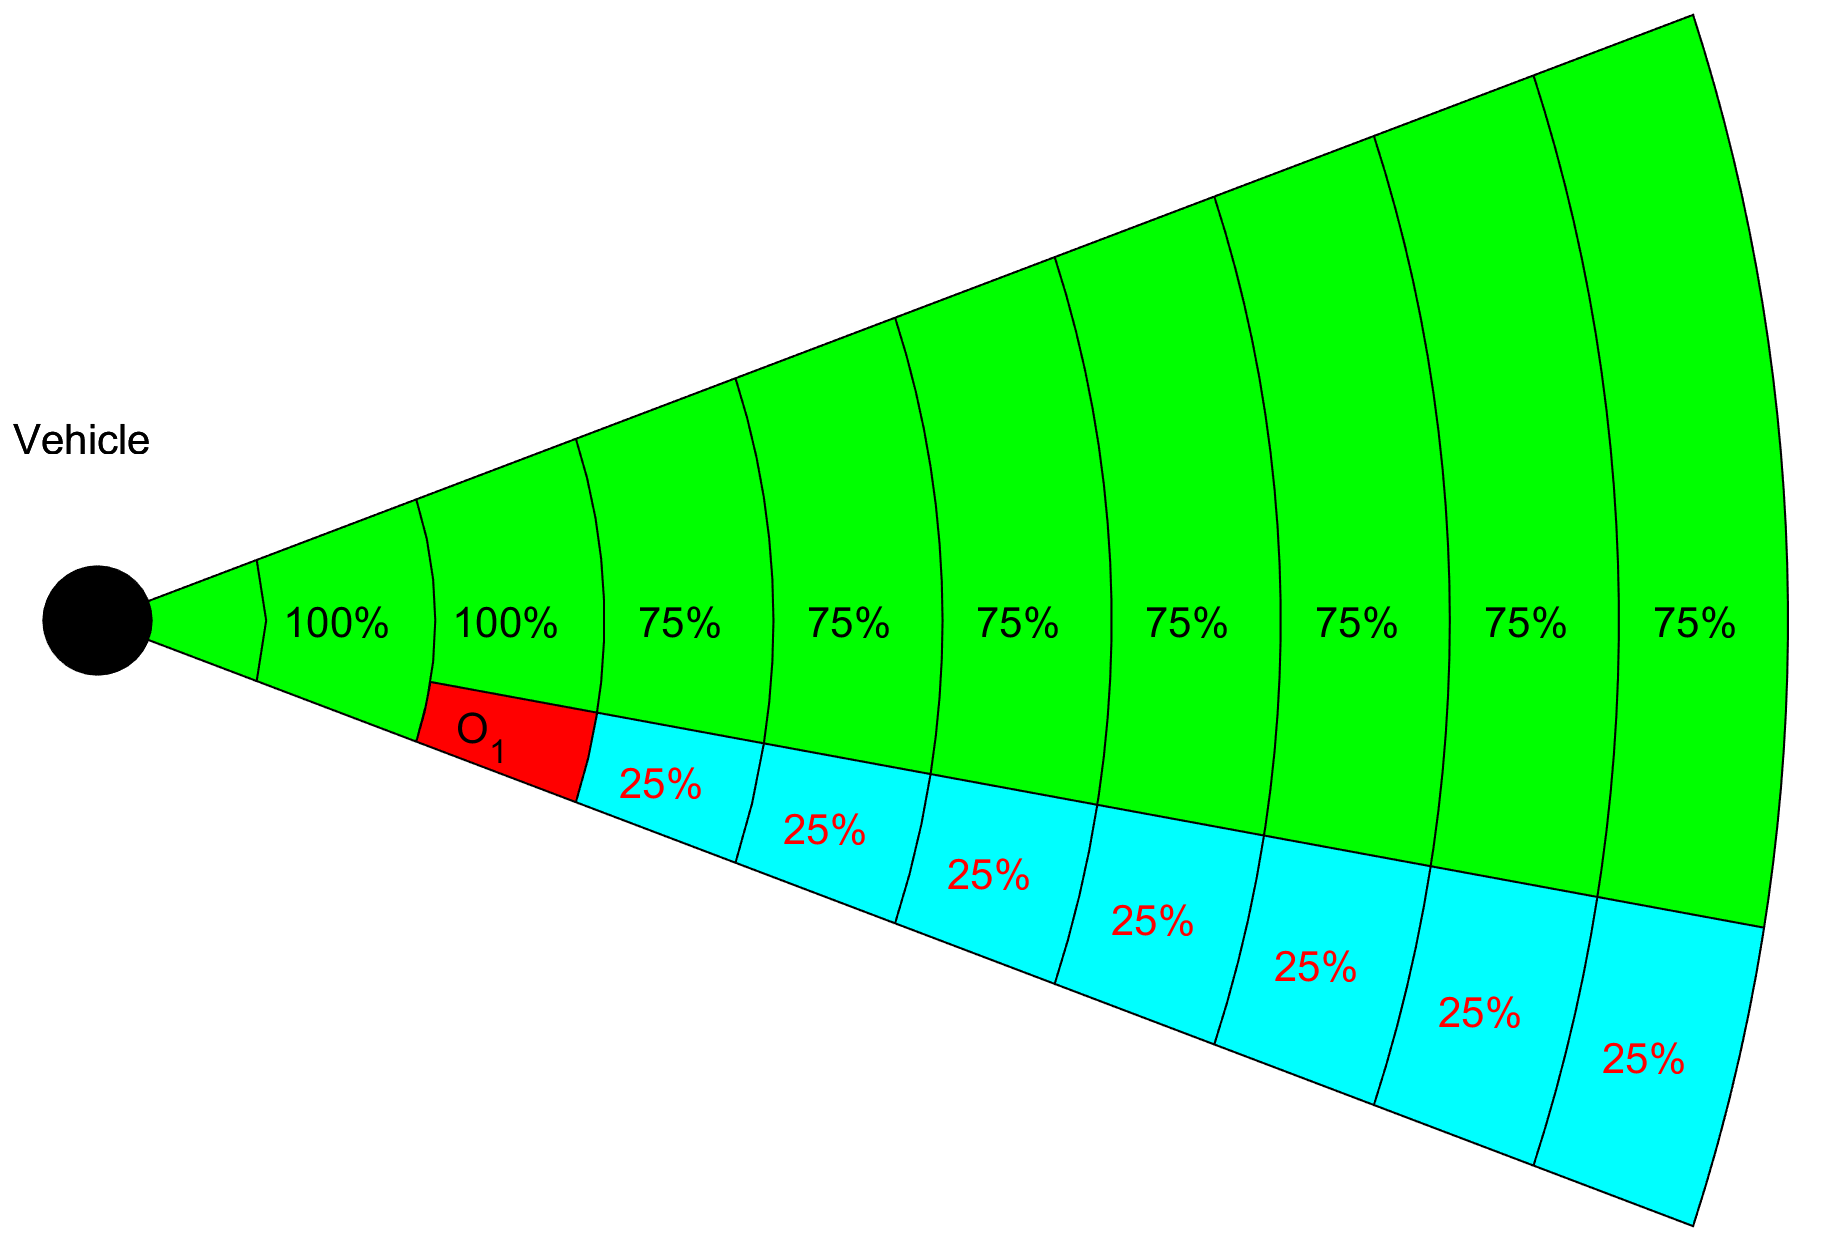
\includegraphics[width=0.9\linewidth]{\FIGDIR/TE006VisibilityFirstObstacle} 
        \caption{1\textsuperscript{st} hindrance.}
        \label{fig:fistObstacleHindrance}
    \end{subfigure}
    \begin{subfigure}{0.32\textwidth}
        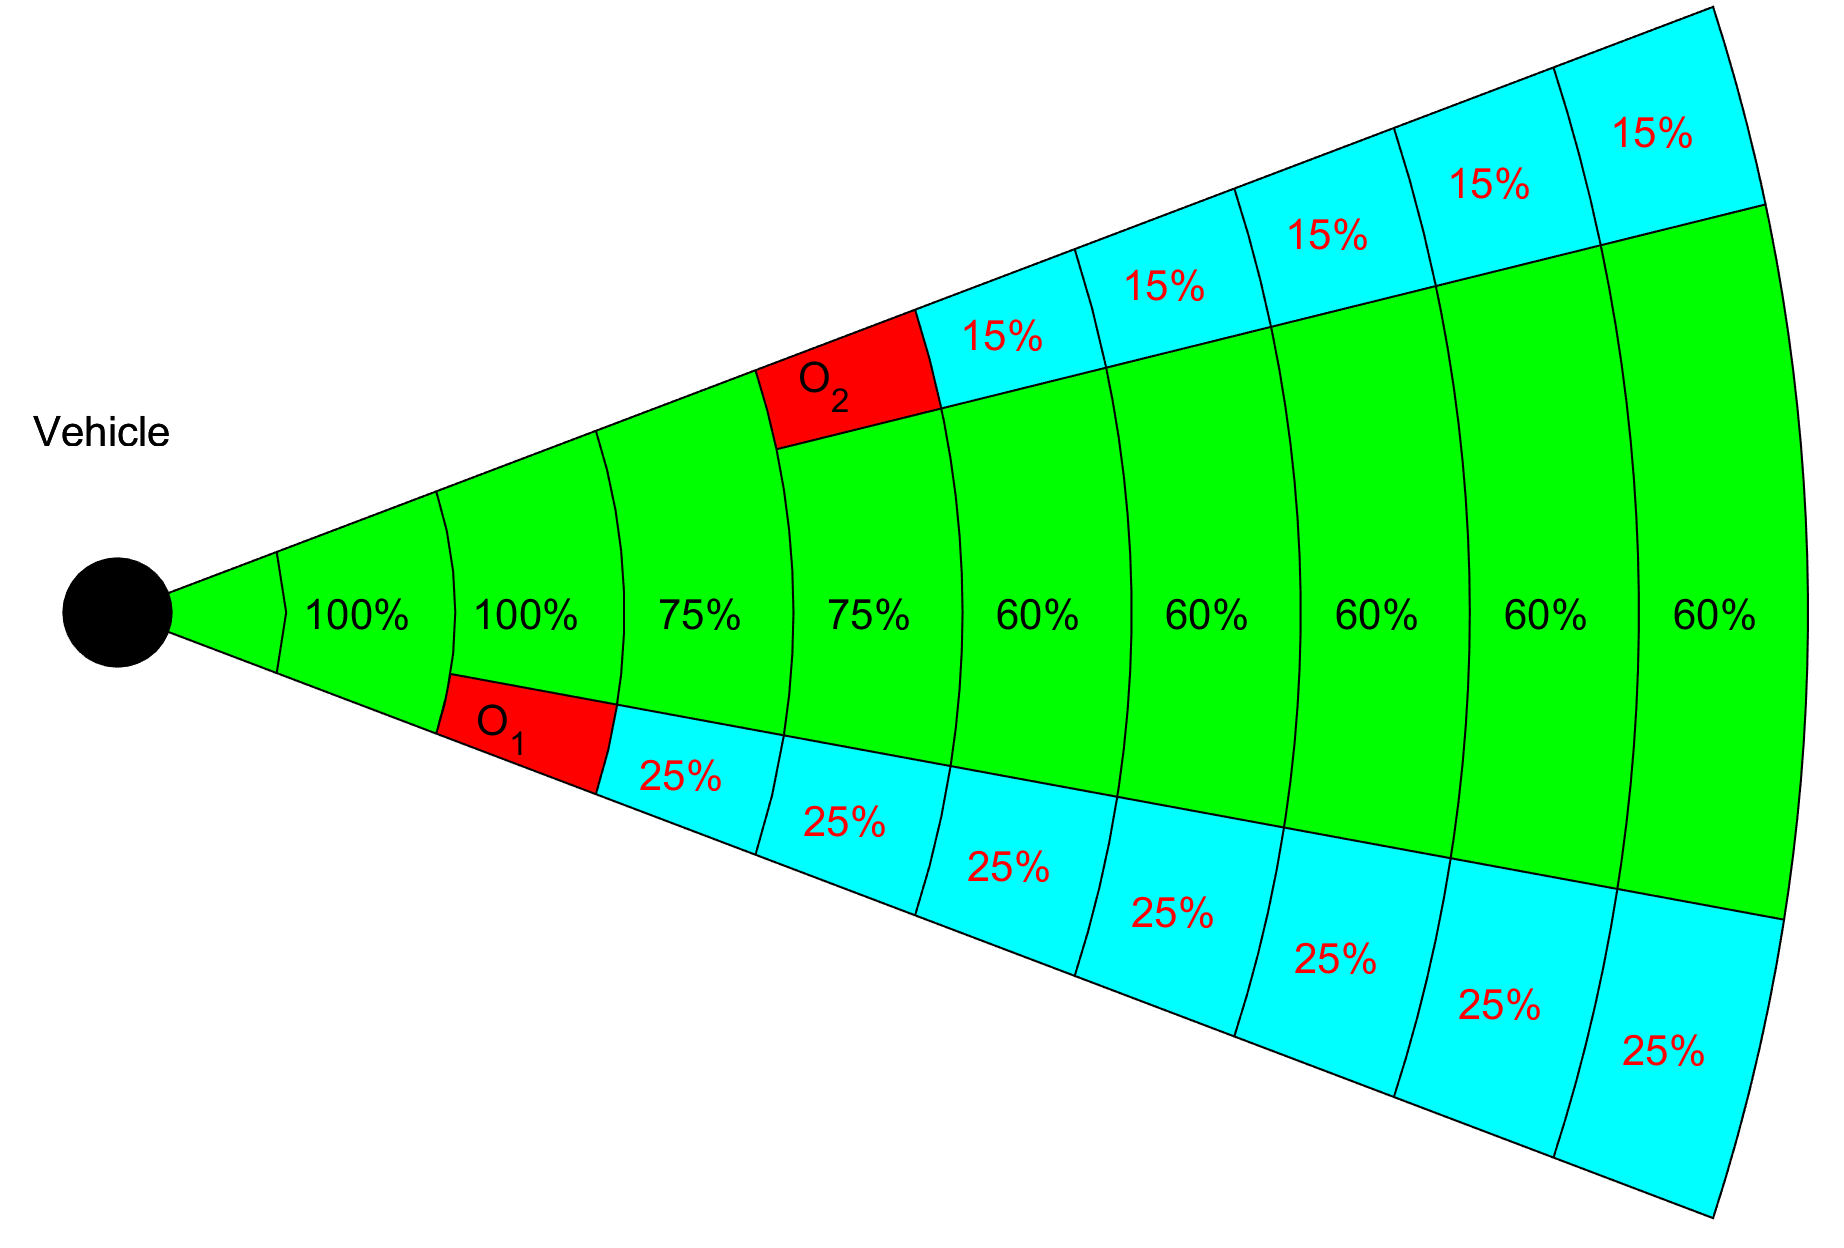
\includegraphics[width=0.9\linewidth]{\FIGDIR/TE007VisibilitySecondObstacle} 
        \caption{2\textsuperscript{nd} hindrance.}
        \label{fig:secondObstacleHindrance}
    \end{subfigure}
    \begin{subfigure}{0.32\textwidth}
        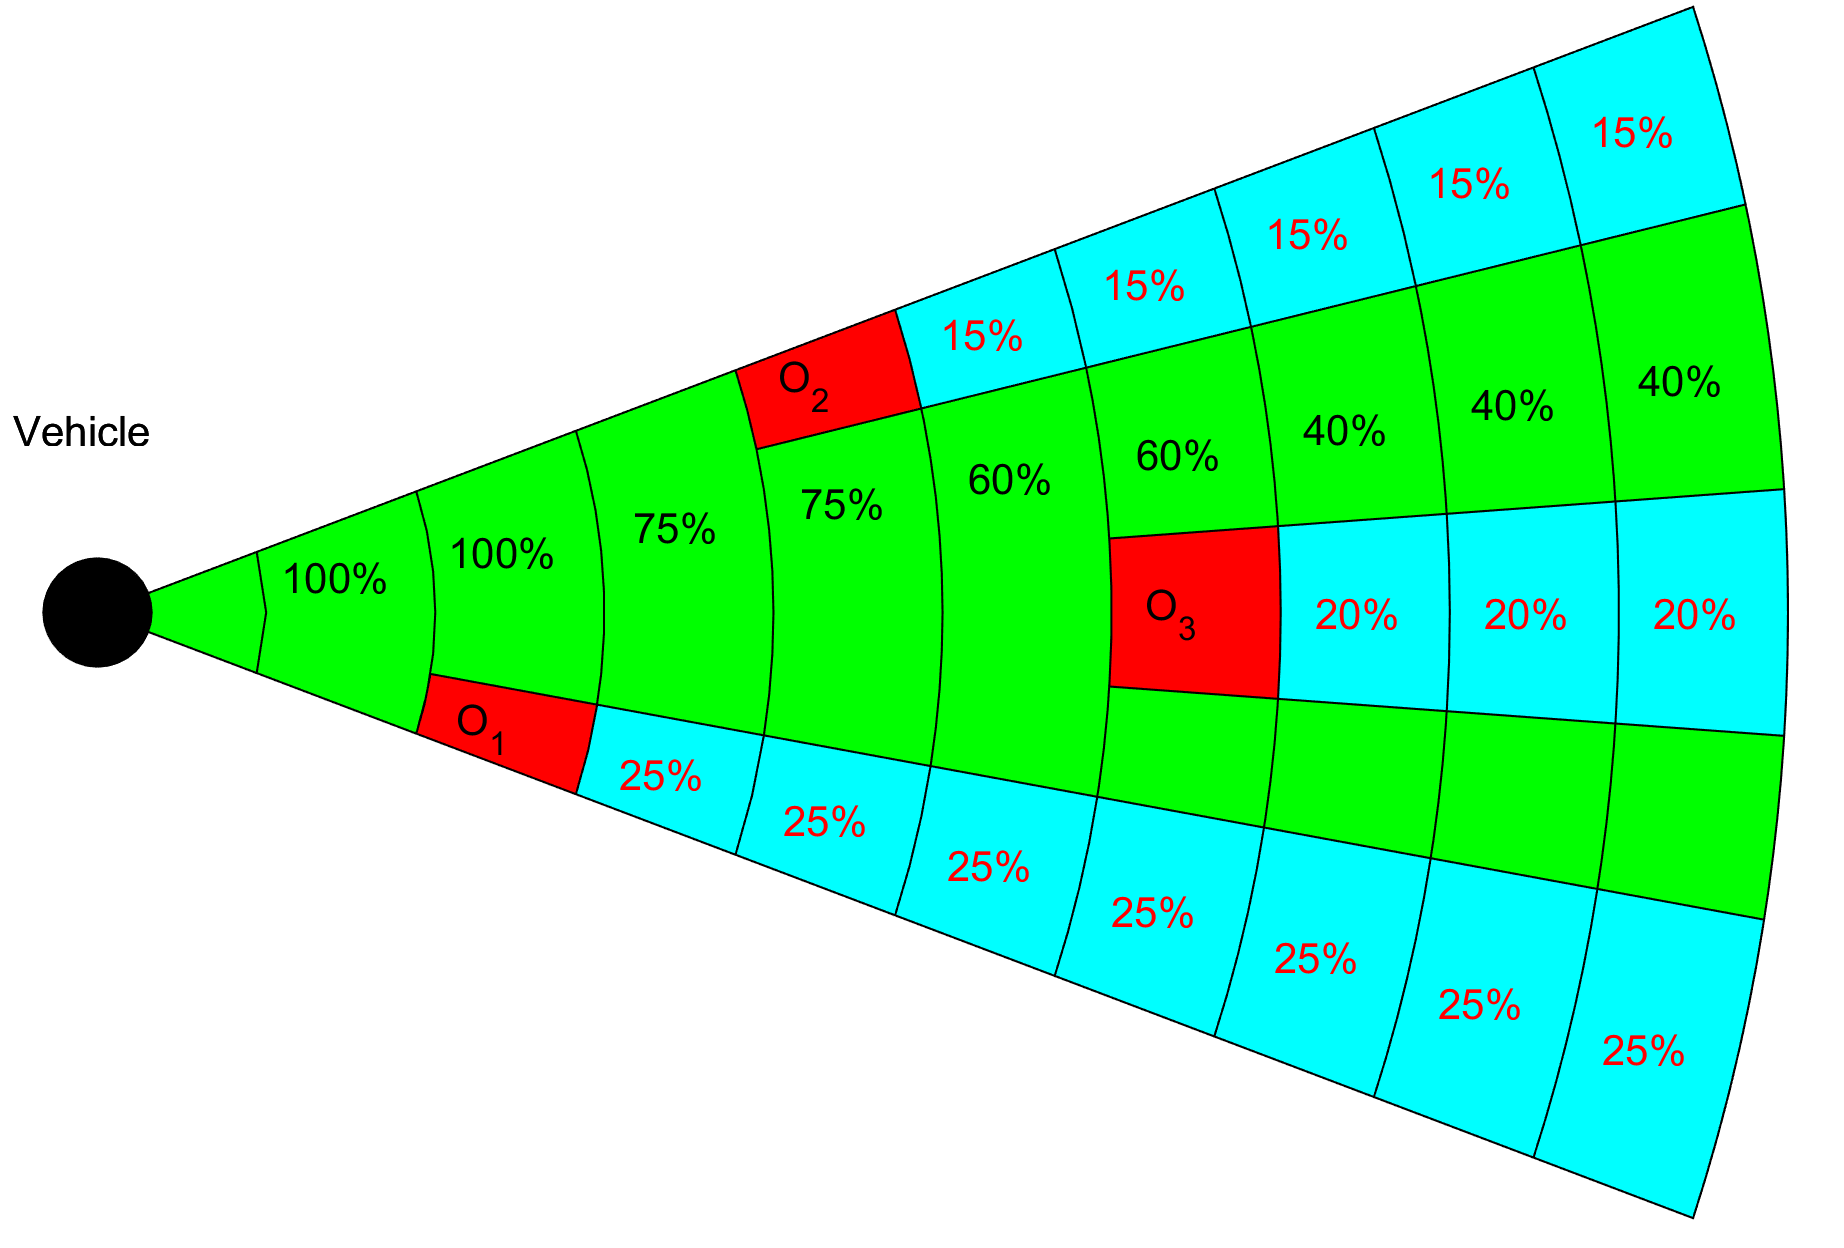
\includegraphics[width=0.9\linewidth]{\FIGDIR/TE008VisibilityThirdObstacle} 
        \caption{3\textsuperscript{rd} hindrance.}
        \label{fig:thirdObstacleHindrance}
    \end{subfigure}
    \caption{Obstacle hindrance impact on visibility in \emph{Avoidance Grid Slice}.}
    \label{fig:hindranceImpactOnVisibility}
\end{figure}

For one cell row $cell Row(j_{fix},k_{fix})$, where count of layers is equal to 10, and layers have equal spacing. There is LiDAR sensor

During consequent LiDAR scans $s(t_0)$, $s(t_1)$, $s(t_2)$, and $s(t_3)$ the obstacle sets $\mathscr{O}_1(t_1)=\{o_1\}$, $\mathscr{O}_2(t_2)=\{o_1,o_2\}$, and $\mathscr{O}_3(t_3)=\{o_1,o_2,o_3\}$ are discovered. Assigned hindrance rates are like follow:

\begin{enumerate}
    \item\emph{Time $t_0$} - there is no obstacle nor hindrance, all cells are fully visible.

    \item\emph{Time $t_1$} (fig. \ref{fig:fistObstacleHindrance}) - $\mathscr{O}_1(t_1)=\{o_1\}$ was detected, the hindrance rate  for $cell_{3,j_{fix},k_{fix}})$ is equal to $0.25$. The visibility rate in cells $cells_{4-10,j_{fix},k_{fix}}$ is $0.75$. 
    
    \item\emph{Time $t_2$} (fig. \ref{fig:secondObstacleHindrance}) - $\mathscr{O}_2(t_2)=\{o_1,o_2\}$ was detected, the additional hindrance rate for $cell_{5,j_{fix},k_{fix}}$ is $0.15$. The visibility rate in  $cells_{6-10,j_{fix},k_{fix}}$ is lowered by additional $0.15$ and its set to $0.60$ now.
    
    \item\emph{Time $t_3$} (fig. \ref{fig:thirdObstacleHindrance}) - $\mathscr{O}_3(t_3)=\{o_1,o_2,o_3\}$  was detected the additional hindrance rate for  $cell_{7,j_{fix},k_{fix}}$ is $0.20$. The visibility rate in $cells_{8-10,j_{fix},k_{fix}}$ is lowered by additional $0.20$ and its set to $0.40$  now.
\end{enumerate}
		%\subsection{\secState{R}Map Obstacles}\label{s:mapObstacles}
\paragraph{Map Obstacles:} Use \emph{stored LiDAR readings} from previous mission to build an compact obstacle map \cite{cernamaria2018}. Then use \emph{this map} as a additional information source.

\begin{figure}[H]
    \begin{subfigure}{0.32\textwidth}
        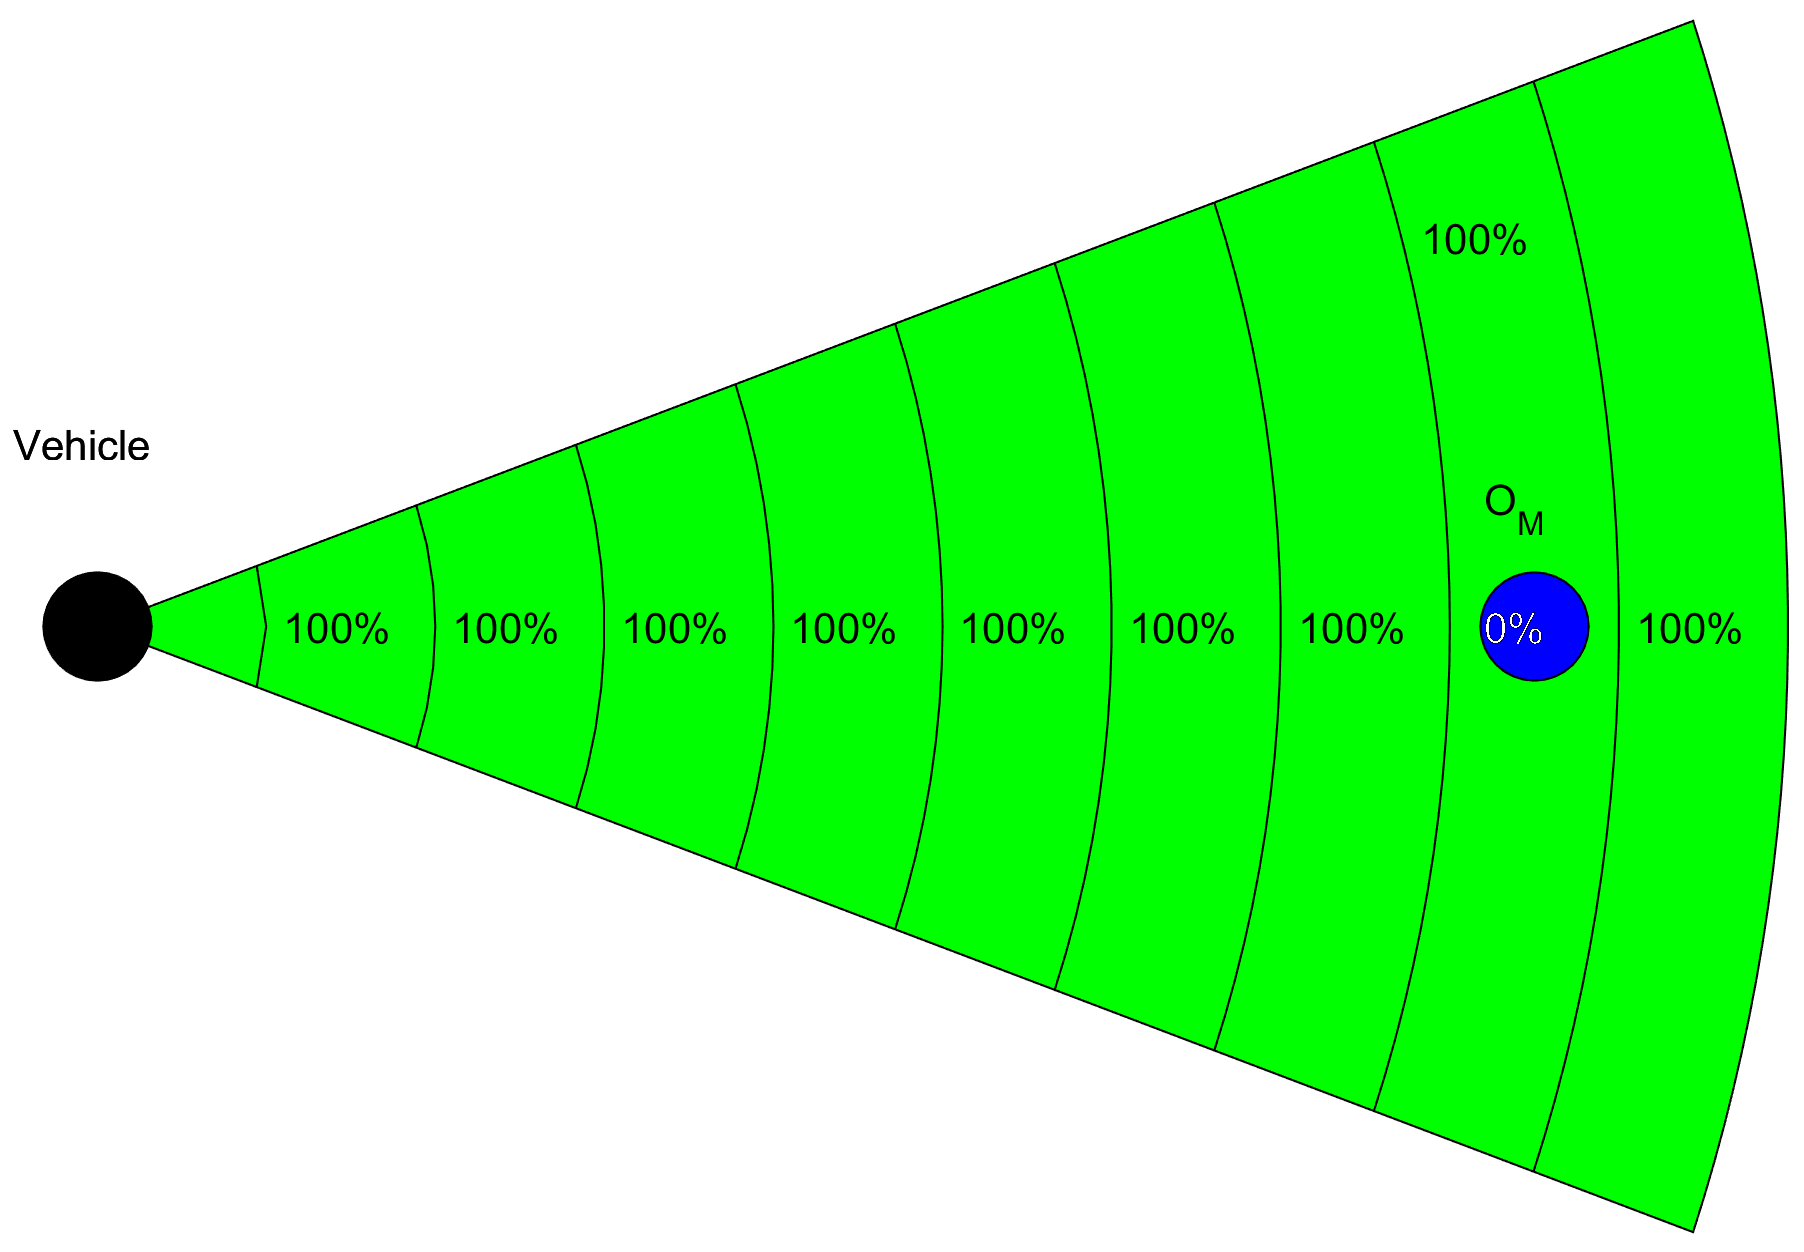
\includegraphics[width=0.9\linewidth]{\FIGDIR/TE009MapObstacleUndetected} 
        \caption{Undetected.}
        \label{fig:undetectedMapObstalce}
    \end{subfigure}
    \begin{subfigure}{0.32\textwidth}
        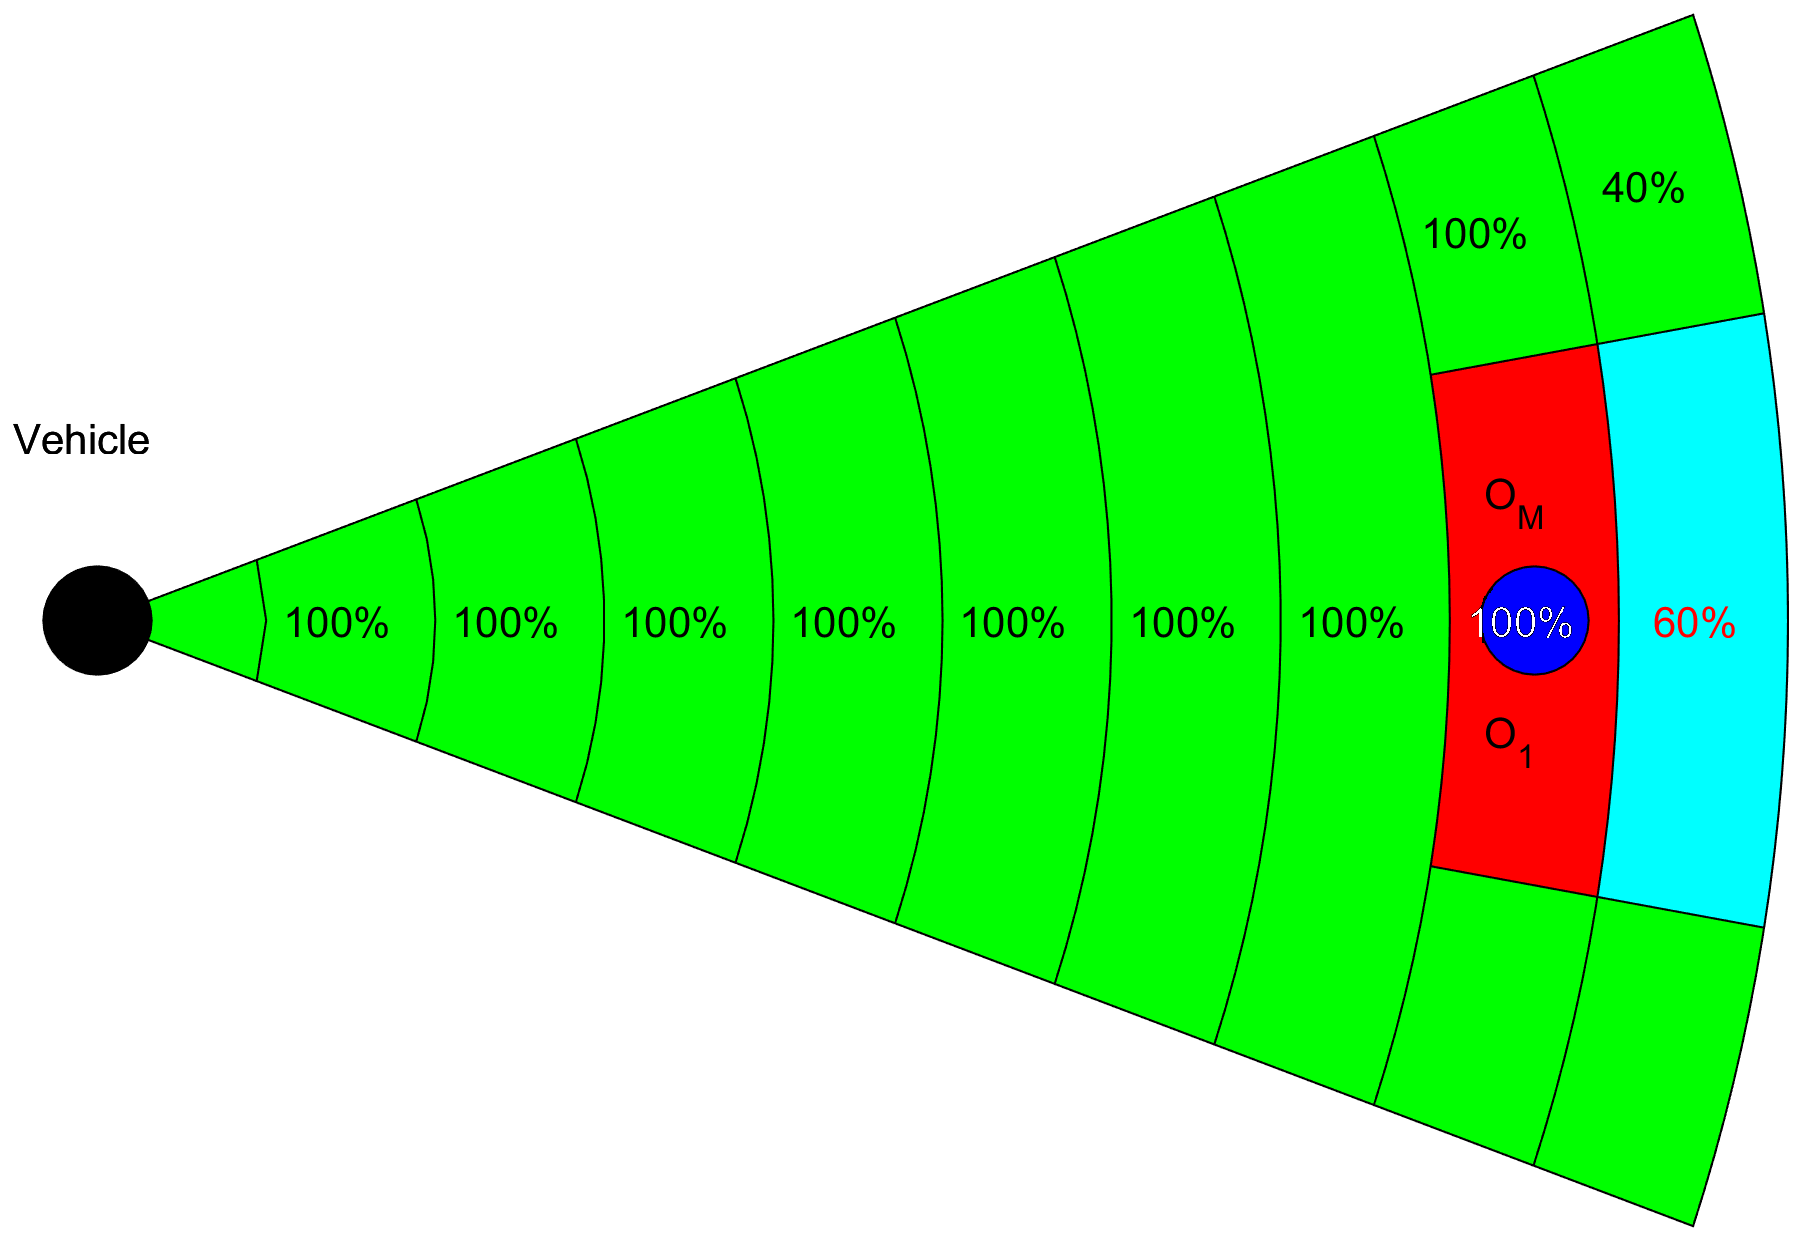
\includegraphics[width=0.9\linewidth]{\FIGDIR/TE010MapObstacleDetected} 
        \caption{Detected.}
        \label{fig:detectedMapObstacle}
    \end{subfigure}
    \begin{subfigure}{0.32\textwidth}
        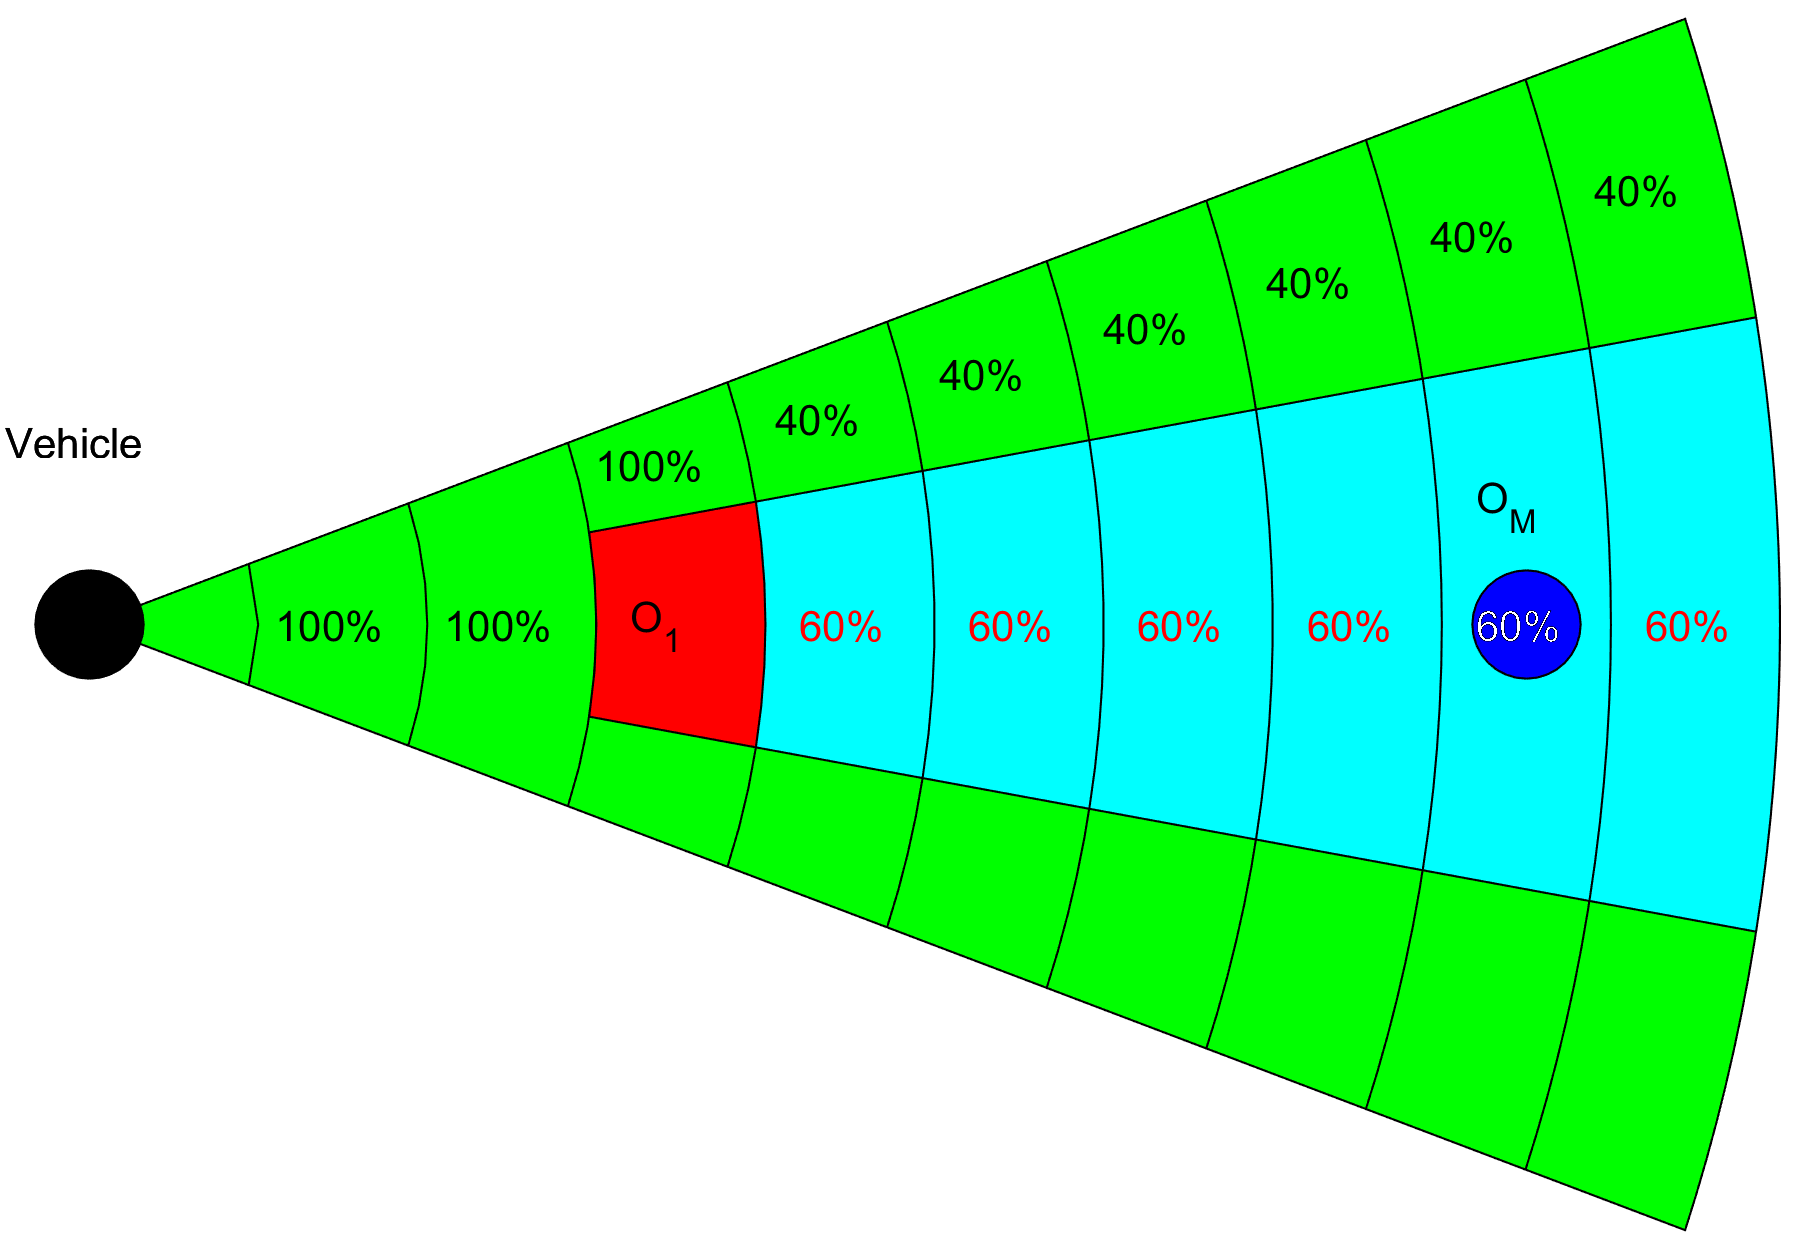
\includegraphics[width=0.9\linewidth]{\FIGDIR/TE011MapObstacleHiden}
        \caption{Hindered.}
        \label{fig:hinderedMapObstacle}
    \end{subfigure}
    \caption{Map obstacle states after \emph{Data fusion}.}
    \label{fig:mapObstacleStatesAfterDataFusion}
\end{figure}

\paragraph{Concept:} A \emph{map obstacle} state has very simple logic, there are three possible cases:

\begin{enumerate}
    \item \emph{Undetected} - Map obstacle $O_M$ is charted on map (fig. \ref{fig:undetectedMapObstalce}), but is undetected by any sensor in sensor field, therefore the probability of map obstacle occurrence is equal to $0$.


    \item \emph{Detected} Map obstacle $O_M$ is charted on map and detected by any sensor in sensor field (fig. \ref{fig:detectedMapObstacle}). The map obstacle rate is equal to detected obstacle rate, usually its equal to $1$.

    \item \emph{Hindered} Map obstacle $O_M$ is hindered behind other detected obstacle $O_1$ (fig. \ref{fig:hinderedMapObstacle}). The detected obstacle $O_1$ is in $cell_{i,j,k}$ and is reducing visibility in follow up $cellRow_{i_f>i,j,k}$ by $60$ percent.
\end{enumerate}

\paragraph{Implementation:} The formulation of final map obstacle rate  $map(cell_{i,j,k})$ was outlined in previous examples. These examples are showing the \emph{desired behaviour} and its solved by \emph{data fusion} (sec. \ref{s:sensorFusion}).

First we start with obstacle map definition. The obstacle map  (eq. \ref{eq:obstacleMap}) defines an map obstacle set of information vectors with position in global coordinate frame , orientation bounded to global coordinate reference frame, safety margin and additional parameters.
\begin{equation}\label{eq:obstacleMap}
    obstacle Map= 
    \left\{
    \begin{bmatrix}
        position,\\
        orientation,\\
        safety Margin,\\
        parameters
    \end{bmatrix}
    :
    \begin{aligned}
        & position \in  \R^3(GCF),\\
        & orientation \in \R^3(GCF),\\
        & safety Margin \in \R^+(m),\\
        & parameters \in \{\dots\}
    \end{aligned}
    \right\}
\end{equation}


The \emph{Map Obstacle} concept is taken from my \emph{master student work} \cite{cernamaria2018}, implementing \emph{compact representation} of point-cloud obstacle map. Te example of \emph{cuboid obstacles} with \emph{safe zone} is given in (fig. \ref{fig:exampleExtractedMapObstacles}).
    
\begin{figure}[H]
    \centering
    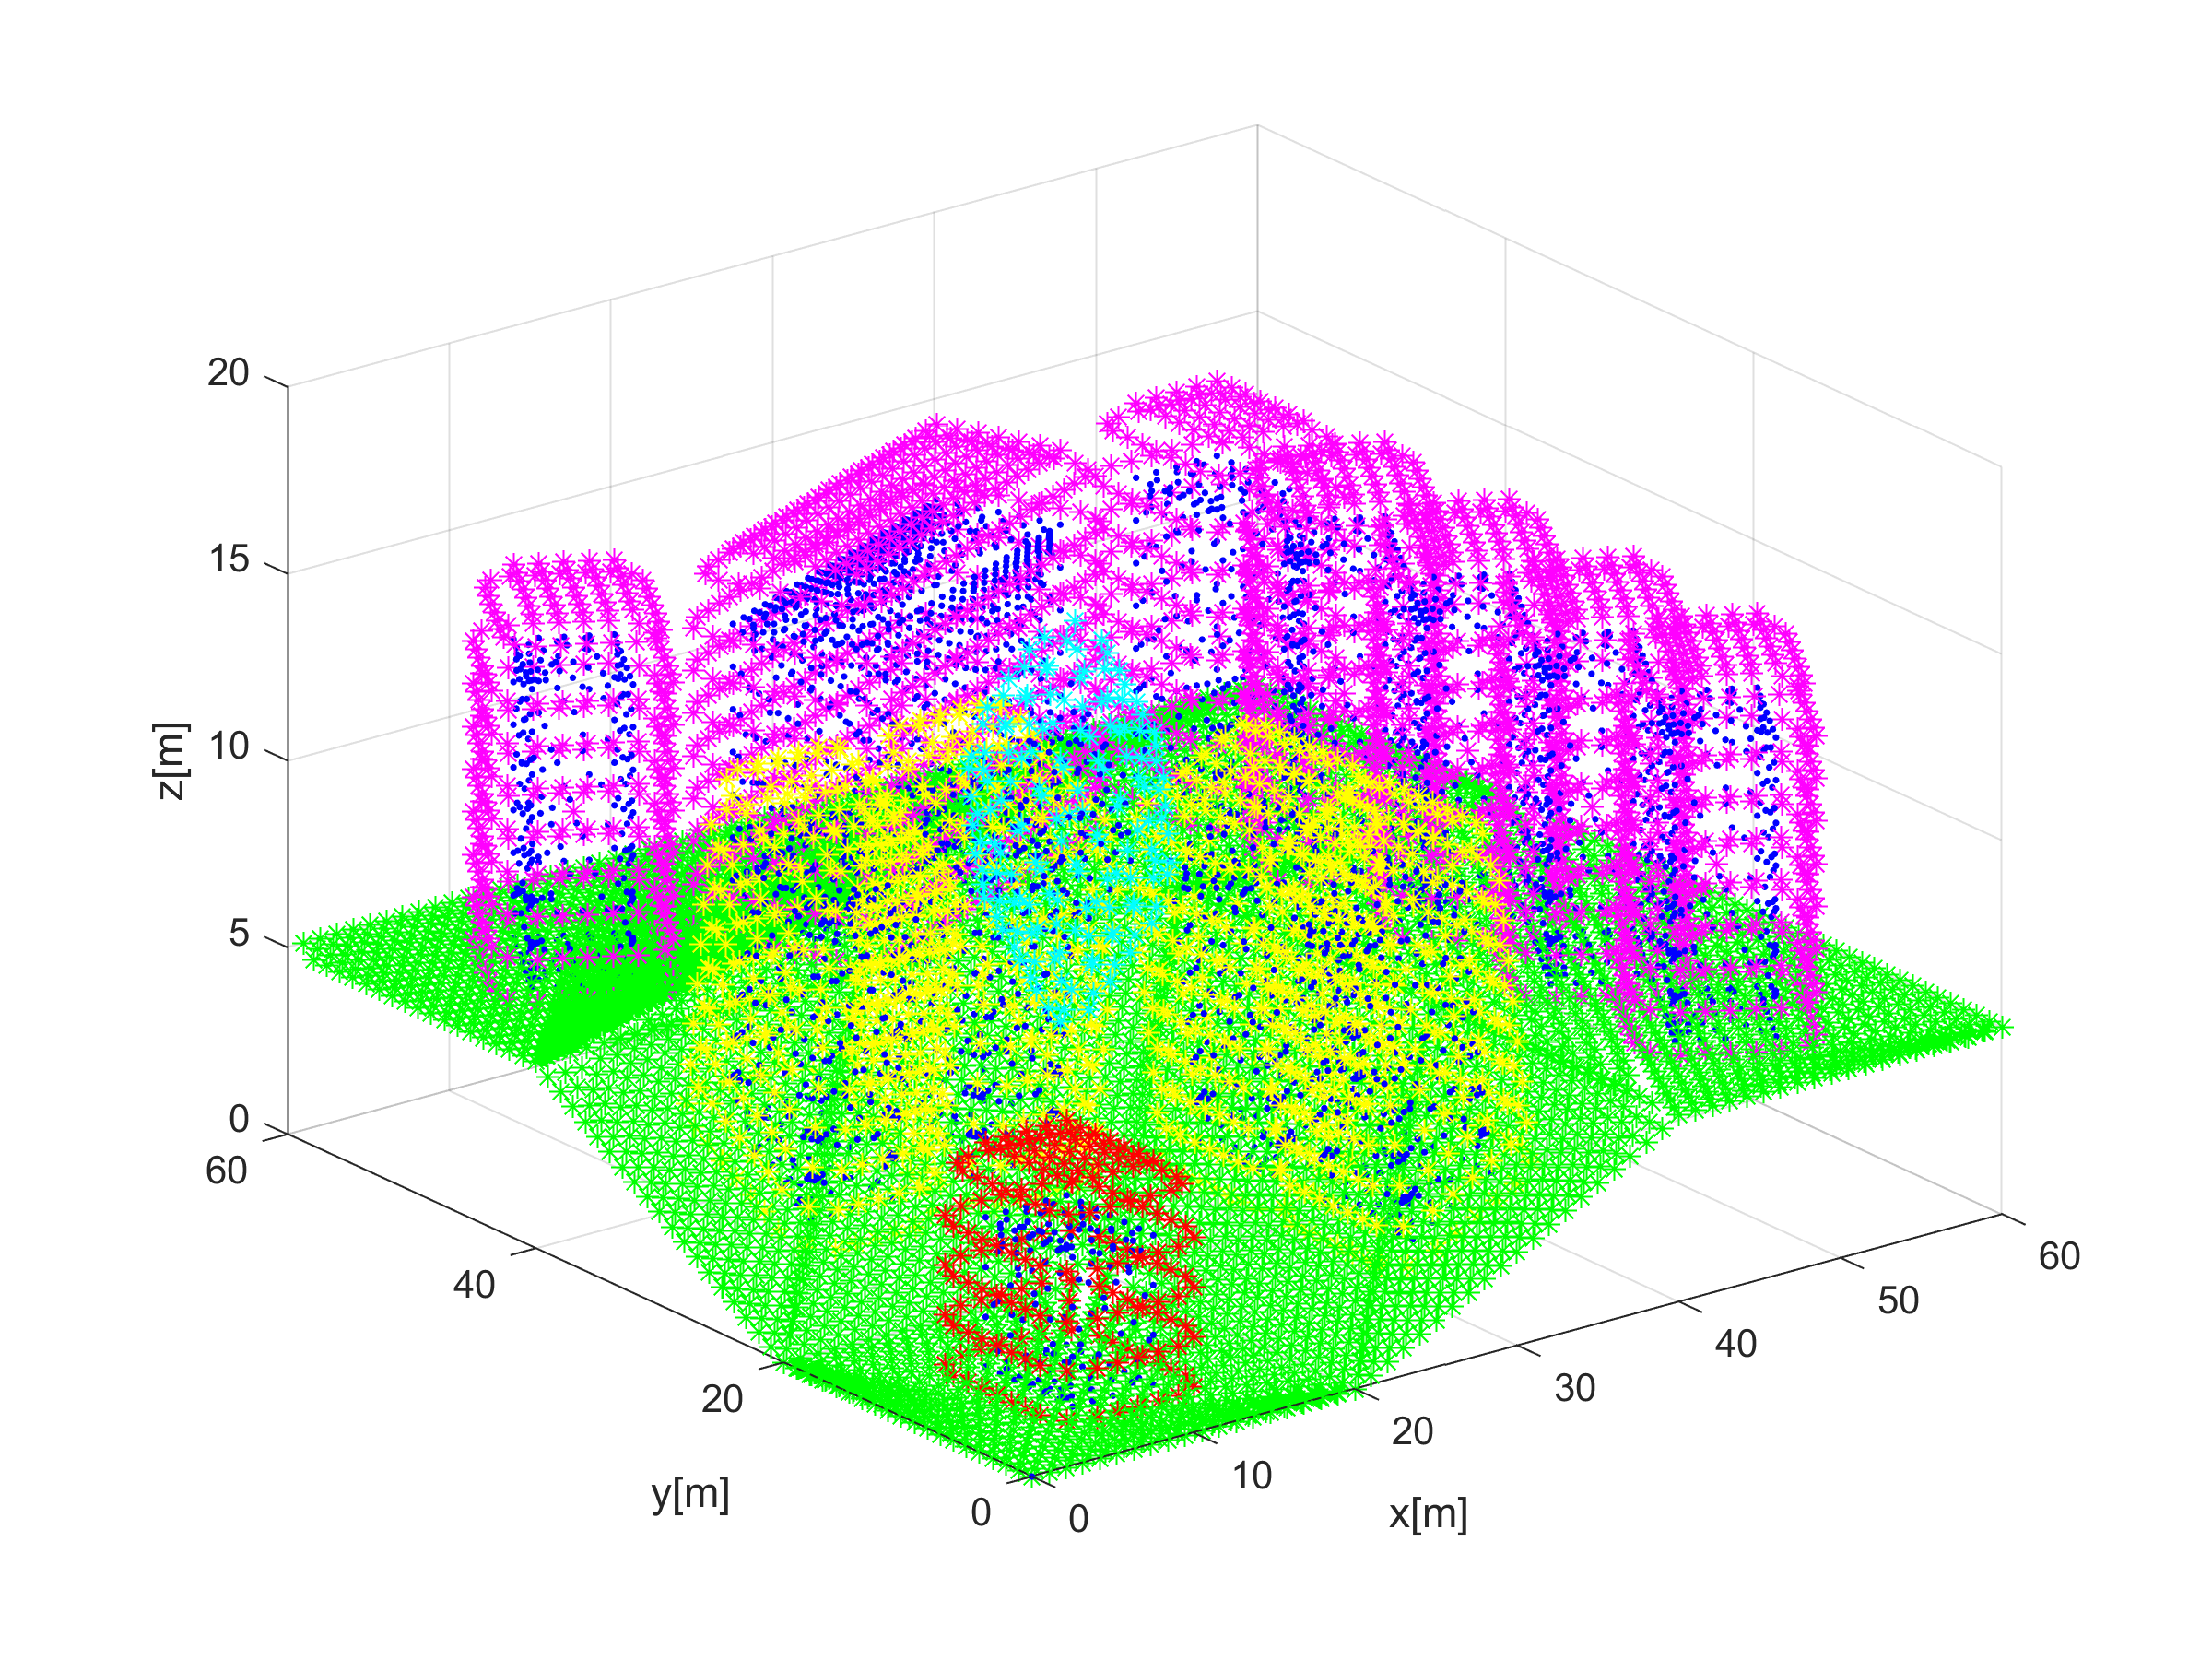
\includegraphics[width=0.7\textwidth]{\FIGDIR/TE054ExtractedMapObstaclesExample}
    \caption{Example of Extracted Map Obstacle \cite{cernamaria2018}.}
    \label{fig:exampleExtractedMapObstacles}
\end{figure} 

\noindent The space covered by any obstacle  is non-empty by definition. There are following types of map charted obstacles which are implemented in framework:

\begin{enumerate}
    \item\emph{Ball obstacle $parameters=\varnothing$} - simple ball with center at $position$, with offset safety margin.
    
    \item\emph{Line obstacle $parameters=[length]$} - simple line bounded by length $\in]0,\infty[$ with center at $position$ and given orientation with respect to main axis in global coordinate frame, with safety margin $<$ 0.
    
    \item\emph{Plane obstacle $parameters=[length,width]$} - bounded rectangle plane partition defined by length $\in]0,\infty[$, and width $w\in]0,\infty[$ with center at $\vec{p}$ and given orientation $\vec{o}$ with respect to main axis in global coordinate frame, with safety margin.
    
    \item\emph{Cuboid obstacle $parameters=[length,width,depth]$} - bounded cuboid space partition defined by length $\in]0,\infty[$, width $\in]0,\infty[$, and depth $d\in]0,\infty[$ with center at $position$ and rotated in orientation with respect to main axis in global coordinate frame, with safety margin.
\end{enumerate}

\noindent The \emph{map obstacles} are stored in clustered database. The \emph{selection criterion} is given in (eq. \ref{eq:mapObstacleSelectionCriterion}).

\begin{equation}\label{eq:mapObstacleSelectionCriterion}
    avoidance Grid.radius \ge distance(UAS.position,map Obstacle) - total Margin
\end{equation}

\noindent The \emph{total margin} is combination of \emph{safety margin} and \emph{body margin} (in case of line, plane, cuboid obstacle). The \emph{selection} was implemented as standard cluster select, selecting 26  surrounding clusters around UAS + own UAS cluster.

\noindent The \emph{compact obstacle representation} is transformed into \emph homogeneous point-cloud representations:

\begin{itemize}
    \item[1.]\emph{Body Point-cloud} - representing obstacle body approximation by geometrical shape (eq. \ref{eq:mapBodyPointCloud}). This point cloud is considered as hard constraints.
    
    \begin{equation}\label{eq:mapBodyPointCloud}
        body Point Cloud  =\{point\in\R^3(GCF): point \in map Obstacle Body\}
    \end{equation}
    
    \item[2.]\emph{Safety Margin Point Cloud} - representing safety coating around mapped obstacle body approximation (eq. \ref{eq:mapMarginPointCloud}). This point cloud is considered as soft constraint.
    \begin{equation}\label{eq:mapMarginPointCloud}
        margin Point Cloud = \{point\in\R^3(GCF): point \in map Safety Margin\}
    \end{equation}
\end{itemize}

\begin{note}
    The \emph{safety margin point cloud} is hollow in relationship to an \emph{body point cloud}, therefore:
    \begin{equation*}
        body Point Cloud \cap margin Point Cloud  = \varnothing
    \end{equation*}
\end{note}

\noindent The \emph{map obstacle} discretization to point cloud leads to problem how to calculate \emph{impact rate}. The \emph{theoretical impact rate} for \emph{obstacle} is given as:
\begin{equation*}
    impact Rate = \frac{volume(map Obstacle\cap cell_{i,j,k})}{volume(cell_{i,j,k})}\in [0,1]
\end{equation*}

\noindent The \emph{map obstacle related point clouds} (eq. \ref{eq:mapBodyPointCloud}, \ref{eq:mapMarginPointCloud}) are homogeneous \cite{cernamaria2018}. That means \emph{each point} in point clouds covers similar portion of object volume. There is \emph{threshold volume} (eq. \ref{eq:tresholdVolumeDefinition}) which represents minimal object volume to be considered as an \emph{obstacle}.

\begin{equation}\label{eq:tresholdVolumeDefinition}
    0< threshold Volume \le \frac{volume(point Cloud)}{|point Cloud|}
\end{equation}

\noindent The \emph{impact rate} of one point  when intersecting a $cell_{i,j,k}$ is given as count of \emph{threshold obstacle bodies} in \emph{point cloud covered mass} multiplied by inverted point count (eq. \ref{eq:pointImpactRateMap}).

\begin{equation}\label{eq:pointImpactRateMap}
    point. rate = \frac{point Cloud Volume}{threshold Volume}\times\frac{1}{|point Cloud|}
\end{equation}

The \emph{intersection set} between \emph{point cloud} and $cell_{i,j,k}$ is defined in (eq. \ref{eq:pointImpactRateMap}). The \emph{cell} intersection with points is defined in (eq. \ref{eq:boundedSpaceCell}).

\begin{multline}\label{eq:pointcloudIntersectionMap}
    intersection(map,cell_{i,j,k}) =\dots\\\dots \{points \in \R^3: (point\to Avoidance Grid Frame) \in cell_{i,j,k}\}
\end{multline}

\newpage \noindent The \emph{map obstacle rating} for $cell_{i,j,k}$ and obstacle for our \emph{information source} is defined in (eq. \ref{eq:mapcellratingourMap}).

\begin{equation}\label{eq:mapcellratingourMap}
    map(cell_{i,j,k},obstacle) =\max\left\{ \sum_{\forall point\in intersection(map,cell_{i,j,k})}  point.rate , 1\right\}
\end{equation}

\noindent The \emph{map obstacle rating} for $cell_{i,j,k}$ and \emph{our information source} is given as maximum of all possible cumulative ratings form each obstacle in \emph{active map obstacles} set (eq. \ref{eq:cumulativeMapCellRatingMap}).

\begin{equation}\label{eq:cumulativeMapCellRatingMap}
    map(cell_{i,j,k} = \max \left\{map(cell_{i,j,k},obstacle):\forall obstacle \in Active Map Obstacles\right\}
\end{equation}

\begin{note}
    The \emph{body point clouds} (eq. \ref{eq:mapBodyPointCloud}) never intersects, because they are created for inclusive obstacles. The \emph{safety margin point clouds} (eq. \ref{eq:mapMarginPointCloud}) can intersects, because they represents protection zones around physical obstacles. Therefore the \emph{maximum obstacle rating} (eq. \ref{eq:cumulativeMapCellRatingMap}) needs to be selected.
\end{note}

		\subsection{Constraints}\label{s:virtualConstraints}
\paragraph{Static Constraints:} The \emph{constraints} (ex. weather, airspace) usually covers a large portion of the \emph{operation airspace}. 

Converting constraints into valued \emph{point-cloud} is not feasible, due to the \emph{huge amount of created points} and low \emph{intersection rate}. The \emph{polygon intersection} or \emph{circular boundary of a 2D polygon} is a simple and effective solution \cite{ritter1990efficient,welzl1991smallest}. 

The key idea is to create \emph{constraint barrels} around dangerous areas. Each \emph{constraint barrel} is defined by a circle on the \emph{horizontal plane} and the \emph{vertical limit range}.

\paragraph{Representation:} The \emph{minimal representation} is based on (sec. \ref{sec:WellClear}, \ref{sec:WeatherImpact}) and geo-fencing principle. The \emph{horizontal-vertical separation} is ensured by \emph{projecting boundary} as 2D polygon oh horizontal plane and \emph{vertical boundary} (barrel height) as \emph{altitude limit}. 

The \emph{static constraint} (eq. \ref{eq:staticConstraint}) is defined as a structure vector including:
\begin{enumerate}
    \item \emph{Position} - the center position in the global coordinates\emph{2D horizontal plane}.
    
    \item \emph{Boundary} - the ordered set of boundary points forming edges in the global coordinates\emph{2D horizontal plane}.
    
    \item \emph{Altitude Range} - the \emph{barometric altitude} range $[altitude_{start},$ $altitude_{end}]$.
    
    \item \emph{Safety Margin} - the \emph{protection zone} (soft constraint) around constraint body (hard constraints) in meters.
\end{enumerate}

\begin{equation}\label{eq:staticConstraint}
    constraint = \{position,boundary, altitude_{start},altitude_{end}, safety Margin\}
\end{equation}

\paragraph{Active constrain selection:} The \emph{active constraints} are constraints which are impacting \emph{UAS active avoidance range}. 

The \emph{active constraints set} (eq. \ref{eq:activeConstraintSet}) is defined as a set of \emph{constraints} from all \emph{reliable Information Sources} where the \emph{distance} between UAS and constraint body (including safety margin) is lesser than the avoidance grid range. The \emph{horizontal altitude range} of avoidance grid must also intersect with \emph{constraint altitude range}.

\begin{multline}\label{eq:activeConstraintSet}
    Active Constraints = \dots\\\dots =
    \left\{\begin{aligned}constraint& \in Information Source:\\ 
    &distance(constraint,UAS) \le Avoidance Grid. distance,\\
    &constraint.altitude Range \cap UAS.altitude Range \neq \varnothing 
    \end{aligned}\right\}
\end{multline}

\paragraph{Cell Intersection:} The \emph{importance of constraints} is on their impact on \emph{avoidance grid} $cells$. The \emph{most of the constraints} (weather, ATC) are represented as 2D convex polygons. Even the \emph{irregularly shaped constraints} are usually split into smaller convex 2D polygons.

The idea is to represent convex polygon boundary as a sufficiently large circle to cover polygon. The Welzl algorithm to find \emph{minimal polygon cover circle} \cite{welzl1991smallest} is used.

First the \emph{set of contraint edges} (eq. \ref{eq:constraintEdgeSet}) is a enclosed set of 2D edges between neighboring points defined as follow:

\begin{equation}\label{eq:constraintEdgeSet}
    edges(constraint) =
    \left\{
    \begin{bmatrix}
        point_{i},point_{j}
    \end{bmatrix}:
    \begin{aligned}
    &point\in boundary,\\
    &i \in \{1,\dots,|boundary|\},\\
    &j \in \{2,\dots, |boundary|,1\}\\
    \end{aligned}
    \right\}
\end{equation}

\noindent The \emph{constraint circle boundary} with calculated center on the  2D horizontal plane and radius (representing body margin) is defined in (eq. \ref{eq:constraintCircleBoundary}).

\begin{equation}\label{eq:constraintCircleBoundary}
    circle(constraint)=
    \left[
        \begin{aligned}
            & center = \frac{\sum boundary.point}{|boundary.point|} + correction\\
            & radius = smallest Circle(edges(constraints)) 
        \end{aligned}
    \right]
\end{equation}

\noindent The $(cell_{i,j,k}$ and \emph{constraint} intersection (eq. \ref{eq:contraintToCellIntersection}) is classification function. The \emph{classification} is necessary, because one \emph{constraint} induce: 
\begin{enumerate}
    \item \emph{Body Constraint} (hard constraint) - the distance between $cell_{i,j,k}$ closest border and \emph{circular boundary} center is in interval $[0,radius]$.
    
    \item \emph{Protection Zone Constraint} (soft constraint) - the distance between $cell_{i,j,k}$ closest border and \emph{circular boundary} center is in interval $]radius,radius+safety Margin]$.
\end{enumerate}


\begin{multline}\label{eq:contraintToCellIntersection}
    intersection,constraint)=\dots\\\dots = 
    \begin{cases}
        hard &:\left[
            \begin{aligned}
                &distance(cell_{i,j,k},circle(constraint)) \le\dots\\ 
                &\quad\dots\le circle(constraint).radius,\\
                & constraint.altitude Range \cap cell_{i,j,k}.altitude Range \neq \varnothing,
            \end{aligned}\right]\\
             &\\
        soft &:\left[
            \begin{aligned}
                &distance(cell_{i,j,k},circle(constraint)) >\dots\\ 
                &\quad\dots > circle(constraint).radius,\\
                &distance(cell_{i,j,k},circle(constraint)) \le\dots\\ 
                &\quad\dots\le circle(constraint).radius + safety Margin,\\
                & constraint.altitude Range \cap cell_{i,j,k}.altitude Range \neq \varnothing,
            \end{aligned}\right]\\
             &\\
        none &:otherwise
    \end{cases}
\end{multline}

\noindent The \emph{intersection impact} of constraint is handled separately for \emph{soft} and  \emph{hard} constraints. The \emph{avoidance} of hard constraints is \emph{mandatory}, the \emph{avoidance} of soft constraints is \emph{voluntary}.

The constraints which have a \emph{soft intersection with the cell} are added to cells impacting constraints set: 
\begin{equation}\label{eq:softConstraintsCellIntersections}
    cell_{i,j,k}. soft Constraints = 
    \left\{
        \begin{aligned}
            &constraint \in Active Constraints:\\ 
            &\quad intersection(cell_{i,j,k},constraint) = soft
        \end{aligned}
    \right\}
\end{equation}

\noindent The constraints which have a \emph{hard intersection with the cell} are added to cells impacting constraints set:

\begin{equation}\label{eq:hardConstraintsCellIntersections}
    cell_{i,j,k}. hard Constraints = 
    \left\{
        \begin{aligned}
            &constraint \in Active Constraints:\\ 
            &\quad intersection(cell_{i,j,k},constraint) = hard
        \end{aligned}
    \right\}
\end{equation}

\begin{note}
    The final \emph{constraint rate value} (eq. \ref{eq:constraintRatingForCell}) is determined based on \emph{mission control run} feed to \emph{avoidance grid} (fig. \ref{fig:missionControlRunActivityDiagram}) defined in  7\textsuperscript{th} to the 10\textsuperscript{th} step.
\end{note}
    

		

%09-Bibliography
    \bibliography{thesis}
\end{document}
